\documentclass[11pt]{article}
\usepackage[margin=1in]{geometry}\usepackage{amsmath,amssymb,amsthm,graphicx,booktabs,hyperref,float}
\newtheorem{prop}{Proposition}\newtheorem{conj}{Conjecture}\theoremstyle{definition}\newtheorem{defn}{Definition}
\newcommand{\hh}{h_2}\newcommand{\wt}{\omega_2}
\title{Exact certification of a paired Jacobsthal bound\\and the dimension-2 sieve barrier:\\a reproducible note on a tightened Goldbach statement}
\author{[Author name] \and Goldbach-Researchs contributors\thanks{Repository: \texttt{github.com/shoblaster/Goldbach-Researchs}. AI-assisted drafting; all numbers are reproducible from the repository.}}
\date{Draft v0.1 --- 10 November 2026 --- \textbf{no proof of Goldbach's conjecture is claimed}}
\begin{document}\maketitle
\begin{abstract}
Ziller and Morack reduce a tightened form of Goldbach's conjecture to a bound $\hh(k)<p_k^2-p_k$ on a paired Jacobsthal function. We (i) re-derive the reduction elementarily, (ii) certify the source's values $\hh(k)$ for $k=3,\dots,10$ (including $\hh(10)=450$) by an exhaustive solver-free search whose infeasibility proofs need up to $2.1\times10^{8}$ nodes, (iii) check the tightened statement for all even $N\in[12,2\cdot10^{7}]$, (iv) tabulate exact fixed-window minima $M_k$, and (v) explain, from source-reported sifting limits, why a standard dimension-2 sieve cannot reach the required range. The bound itself remains \emph{unproved} for all $k$; rows $k\ge 11$ are transcribed. Novelty of every item is \textbf{not} established; see Section~\ref{sec:limits}.
\end{abstract}

\section{Setting}
Let $p_k$ be the $k$-th prime. For $k\ge3$, $\hh(k)$ is the least $m$ such that for every pair $(a,b)$ with $2\mid(b-a)$ some $q\in\{1,\dots,m\}$ makes both $a+q$ and $b+q$ coprime to $p_1\cdots p_k$ \cite{ZM1,ZM2}. Equivalently, $\hh(k)=6\wt(k)+6$, where $\wt(k)$ is the largest $L$ such that one can choose \emph{two} nonzero residues modulo each prime $p\in\{5,\dots,p_k\}$ (one class mod 2, by the source's normalisation) covering all positions $1,\dots,L$ \cite{ZM3}. We use the source's equivalence as stated and verify it only through direct witness re-checks (Section~\ref{sec:comp}).
\begin{conj}[H; source Conjecture 6]\label{c:H} $\hh(k)<p_k^2-p_k$ for all $k\ge3$.\end{conj}
\begin{conj}[Tightened Goldbach; source Conjecture 4]\label{c:4} For even $N\ge12$ with $p_k^2+p_k\le N<p_{k+1}^2+p_{k+1}$ there are primes $q_1,q_2$, $p_k<q_1<p_k^2$, $q_1+q_2=N$.\end{conj}

\section{The reduction}
\begin{prop}[source Prop.~3.2, re-derived]\label{p:red} For $k\ge3$, if $\hh(k)\le p_k^2-p_k-1$ then Conjecture~\ref{c:4} holds for every even $N$ with $p_k^2+p_k\le N<p_{k+1}^2+p_{k+1}$.\end{prop}
\begin{proof} Put $p=p_k$ and take $(a,b)=(p,\,p-N)$; $b-a=-N$ is even. There is $q\le p^2-p-1$ with $p+q$ and $p-N+q$ both coprime to $p_1\cdots p_k$. Let $q_1=p+q$, $q_2=N-q_1$. Then $p<q_1<p^2$ and $q_1$ has no prime factor $\le p$, so it is prime ($q_1<p^2$). Next $q_2\ge p^2+p-(p^2-1)>1$ has no prime factor $\le p$, and $q_2\le N-p_{k+1}<p_{k+1}^2$, so $q_2$ is prime.\end{proof}
Hence Conjecture~\ref{c:H} implies Conjecture~\ref{c:4} for $k\ge3$; the range $12\le N\le29$ ($k=2$) is a finite check. The source's case split is written with thresholds in $n=N/2$ that behave like thresholds in $N$; this is a harmless boundary slip (repository note \texttt{PROOF\_FRONTIER\_022} \S3; read from the arXiv text via web extraction, not a local PDF).

\section{Exhaustive certification of $\hh(k)$ for $k\le10$}\label{sec:comp}
\paragraph{Method.} For fixed $(k,L)$ we search for a choice of two classes per prime covering $[1,L]$ by depth-first search: branch on the lowest uncovered position $q$ and on which prime covers it with residue $q\bmod p$, pruning when an exact upper bound on the coverage still obtainable falls short. Certification of $\hh(k)=H$ means: $L=\wt(k)$ is feasible (witness re-verified directly against the definition) and $L=\wt(k)+1$ is infeasible (search exhausted). No MILP/SAT solver is used. A parallel variant splitting at depth 2 gives identical infeasible node counts for $k=5,\dots,10$.
\begin{table}[H]\centering\small\setlength{\tabcolsep}{4pt}\setlength{\tabcolsep}{4pt}
\begin{tabular}{rrrrrrr}\toprule $k$&$p_k$&$\hh(k)$&$\wt$&$p_k^2-p_k$&ratio&status\\\midrule
3&5&18&2&20&0.900&certified\\4&7&30&4&42&0.714&certified\\5&11&66&10&110&0.600&certified\\6&13&150&24&156&\textbf{0.962}&certified\\7&17&192&31&272&0.706&certified\\8&19&258&42&342&0.754&certified\\9&23&366&60&506&0.723&certified\\10&29&450&74&812&0.554&certified\\11--21&31--73&570--2622&&&$\le0.62$&transcribed\\\bottomrule\end{tabular}
\caption{Values from \cite{ZM1} Table 1; certified rows re-derived by exhaustive search (repository EXP030; $\hh(10)$ also by an independent implementation, EXP029, same algorithm family). Full data: \texttt{data/h2\_table.csv}.}\end{table}
\begin{figure}[H]\centering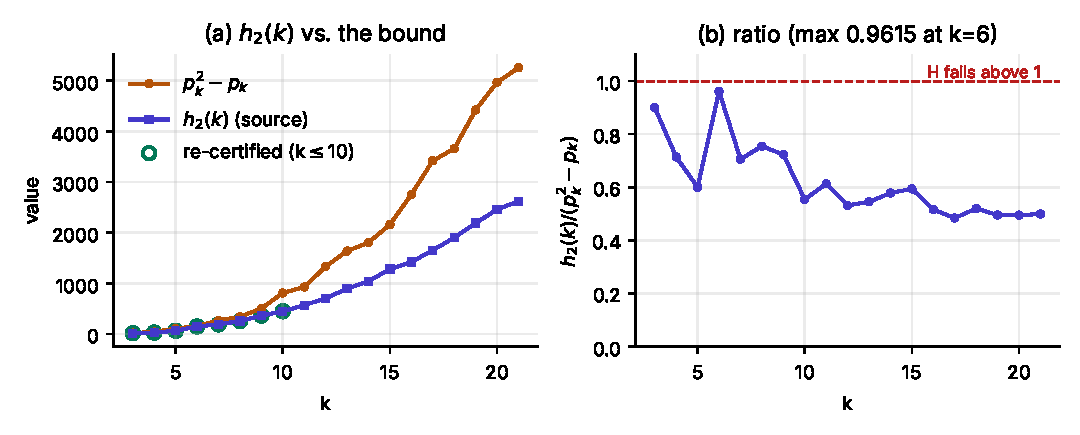
\includegraphics[width=\linewidth]{figures/fig1_h2_vs_bound.pdf}\caption{(a) $\hh(k)$ against $p_k^2-p_k$; circles mark certified rows. (b) The ratio never exceeds $0.9615$ ($k=6$), so Conjecture~\ref{c:H} holds on all 19 tabulated rows, but the margin at $k=6$ is only $6$.}\end{figure}
\begin{figure}[H]\centering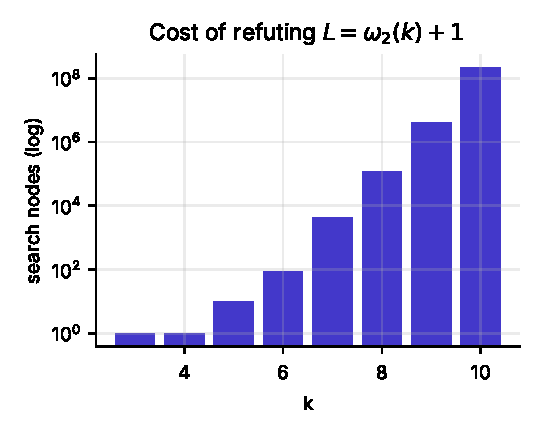
\includegraphics[width=.49\linewidth]{figures/fig2_search_nodes.pdf}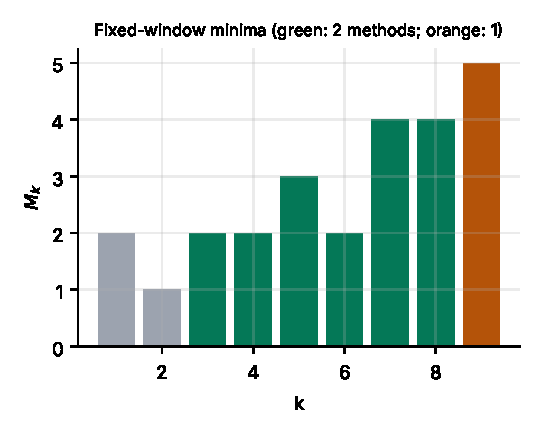
\includegraphics[width=.49\linewidth]{figures/fig3_mk.pdf}\caption{Left: nodes to refute $L=\wt(k)+1$ for $k=3..10$ (exact counts in \texttt{data/infeasibility\_nodes.csv}; $2.1\times10^{8}$ at $k=10$), growth $\approx\times30$--$50$ per step. Right: exact fixed-window minima $M_k$ (survivors in $[1,p_k^2]$ with one class mod 2 and two mod each odd prime); $k\le8$ confirmed by two independent methods, $M_9=5$ by one.}\end{figure}
\paragraph{Not obtained.} $k=11$: the lower bound ($\wt\ge94$) holds, but the infeasibility run at $L=95$ ended without a result; we record \emph{no result}.

\paragraph{Finite check of Conjecture~\ref{c:4}.} All $9{,}999{,}995$ even $N\in[12,2\cdot10^{7}]$ pass; an independent trial-division check for $N\le10^{5}$ agrees (EXP023). This is evidence, not proof.

\section{A dimension-2 sieve barrier (heuristic)}
The covering window has length $\approx p_k^2$ and sifts by all primes $\le p_k\approx x^{1/2}$ with two classes removed per prime, i.e.\ sieve dimension $\kappa=2$. A lower-bound sieve of dimension $\kappa$ gives a positive count only when the sifting level satisfies $z\le x^{1/\beta_\kappa}$ with $\beta_2$ the sifting limit; Franze reports $\beta_2=4.266$ (Diamond--Halberstam--Richert) and $4.516$ ($\Lambda^2\Lambda^-$), and cites $\beta_2<4.45$ (Blight) \cite{Fra}. Thus the reachable range is $z\le x^{0.234},x^{0.225},x^{0.221}$, short of the $x^{1/2}$ required (Fig.~\ref{fig:sv}). This is an argument by comparison with source-reported constants---not a theorem---and the parity problem \cite{Ford} is the underlying obstruction. A bound of the Iwaniec type for the ordinary Jacobsthal function \cite{CW} would settle the order of $\hh$ only if its constant is explicit and small; a paired analogue is not known to us.
\begin{figure}[H]\centering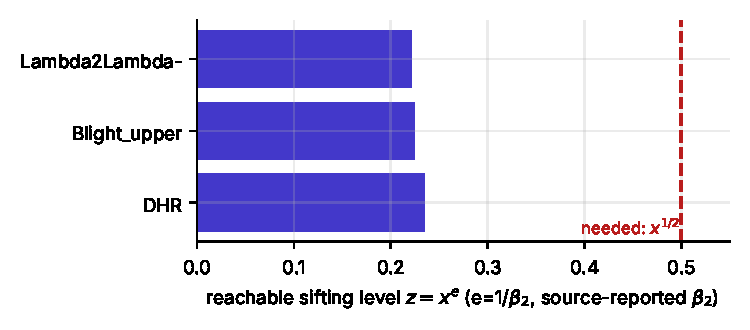
\includegraphics[width=.7\linewidth]{figures/fig4_sieve_barrier.pdf}\caption{Reachable sifting exponent $1/\beta_2$ vs.\ the $x^{1/2}$ requirement. The $\beta_2$ values are \emph{source-reported and not re-derived}.}\label{fig:sv}\end{figure}

\section{Reproducibility}
Every figure is produced by \texttt{11\_PAPER/make\_figures.py} from the CSVs in \texttt{11\_PAPER/data/}; \texttt{verify\_data.py} recomputes $p_k$, checks $\hh(k)=6\wt+6$, $\hh<p_k^2-p_k$, and re-runs the search for $k\le8$, matching the node counts (about one minute on one core). Larger rows use \texttt{03\_CODE/h2\_cover\_search(\_par).cpp} (repository branch history; raw output in \texttt{06\_EXPERIMENTS/EXP030*}). The parallel $k=10$ run takes about 21\,s.

\section{Limitations and requests for review}\label{sec:limits}
(1) Conjecture~\ref{c:H} is unproved for all $k$; $k\ge11$ is transcribed. (2) The certification trusts the covering-model equivalence from \cite{ZM3}; both implementations share one algorithm, so agreement is an implementation, not a method, cross-check. (3) $M_9$ rests on one solver run. (4) The $\beta_2$ values and the sieve comparison need checking against the primary books. (5) Novelty is not established. We would value a pointer to prior work on exact $\hh(k)$ or on paired-progression covering bounds, and on whether a structural route (symmetry, density of the extremal covers) could beat brute force beyond $k=11$.

\begin{thebibliography}{9}
\bibitem{ZM1}M.~Ziller, J.~F.~Morack, \emph{A short note on the computation of the generalised Jacobsthal function for paired progressions}, arXiv:1706.03668 (2017).
\bibitem{ZM2}M.~Ziller, J.~F.~Morack, \emph{Divisibility in paired progressions, Goldbach's conjecture, and the infinitude of prime pairs}, arXiv:1706.00317 (2017).
\bibitem{ZM3}M.~Ziller, J.~F.~Morack, ancillary file \emph{On the computation of the generalised Jacobsthal function for paired progressions}, arXiv:1706.03668v1.
\bibitem{CW}L.~Costello, D.~Watts, \emph{A short note on Jacobsthal's function}, arXiv:1306.1064 (2013).
\bibitem{Fra}C.~Franze, \emph{Sifting limits for the $\Lambda^2\Lambda^-$ sieve}, arXiv:1012.3809 (2010).
\bibitem{Ford}K.~Ford, \emph{On Bombieri's asymptotic sieve}, arXiv:math/0401215.
\end{thebibliography}
\end{document}
